\documentclass{article}

\usepackage{subcaption}
\usepackage{amsmath}
\usepackage{color}
\usepackage{xcolor}
\usepackage{graphicx}
\usepackage{caption}
\usepackage{float}
\usepackage[hidelinks]{hyperref}
\usepackage{enumitem}
\usepackage[bottom]{footmisc}
\usepackage[margin=.8in, tmargin=.5in]{geometry}
\setlength\parindent{0pt}
\captionsetup{justification=centering}

\title{Computer Science Large Practical Report}
\date{Tue, 20 Dec 2016}
\author{Traiko Dinev \textless s1448355\textgreater}

\begin{document}
	\maketitle

    \section{Introduction}
		This report describes the simulator of a bin collection process in a city, as described here (\url{http://www.inf.ed.ac.uk/teaching/courses/cslp/handout/cslp-2016-17.pdf}).
	
	\section{Simulator Architecture}
		The simulator has a decouple, observer pipeline, where everything is governed by an \textit{EventDispatcher} that schedules
		\textit{Events} and calls attached \textit{Observers}. The \textit{Areas}, the \textit{StatisticsAggregator} as well as the
		\textit{OutputFormatter} all have observers that listen to events happening. This way the output functionality and the statistics
		operate purely on the events happening and have no knowledge of the rest of the system, making them easier to develop and maintain.
		\\ \\
		See Figure~\ref{fig:fig1} for more details. The \textit{ExperimentManager} class creates one \textit{OutputFormatter}, \textit{StatisticsAggregator}
		and \textit{Simulation} and uses them for all runs necessary.

		\begin{figure}[H]
		\centering
			\includegraphics[width=.8\columnwidth]{resources/architecture.png}
			\captionof{figure}{Project Architecture \\\textit{file: resources/architecture.png}}
			\label{fig:fig1} 
		\end{figure}

	\subsection{Simulation Runs and Experiments}
		Each \textbf{run} of the program is governed by an \textit{ExperimentManager}, where actual experimentation behaves identically, while
		disabling detailed output (by not attaching an \textit{OutputFormmater} to the dispatcher.
		\\
		\\
		As such, each experiment contains a single \textit{Simulation}, which contains as many \textit{Area}s as necessary.
		Each \textit{Area} listens to events that happen in it and reacts accordingly. It also registers new disposal events and service events,
		as well as lorry events. Note the algorithm itself is separated and injected as a dependency in the constructor of the \textit{Area} class, thus
		separating that functionality out.


		\subsubsection{Pipeline}
		The input parser is the starting point of the application. Once we get a valid configuration file from the parser, we instantiate the
		\textit{ExperimentManager} class, which is in charge of creating each \textit{Simulation}, which create \textit{Areas}, which contain the actual
		simulation code. To glue things together, the \textit{EventDispatcher} is injected in the constructor of the Simulation, which in turn 
		injects it into each area class. Statistics and output are achieved similarly. The \textit{EventDispatcher} class is injected into an
		\textit{OutputFormatter} and into a \textit{StatisticsAggregator} class.
			\\
			\\
			See Figure~\ref{fig:fig2} for a sequence diagram illustrating the start of the simulation and a cycle of events.

		\begin{figure}[H]
		\centering
			\includegraphics[width=1\columnwidth]{resources/start_sequence.png}
			\captionof{figure}{Startup Sequence \\\textit{file: resources/start\_sequence.png}}
			\label{fig:fig2} 
		\end{figure}

	\subsection{Route Planning}
	Route planning is done separately in the \textbf{DijkstraRoutePlanner} class. The route planner uses Dijkstra's algorithm each time
	a route is needed and two different heuristics for selecting the next bin to be serviced. The \textit{greedy} algorithm always services
	bins according to their occupancy (or volume). The \textit{priority} algorithm always services the closest bin. Both always use only the bins
	that need servicing (i.e. they do not ever calculate a path that would empty a bin that has not exceeded the occupancy threshold).

	\subsection{Optimization} \label{optimization}
		The greedy algorithm is generally faster than the priority algorithm and hence the default setting of the algorithm it \textit{dynamic}, which
		selects one of the two versions based on how many bins are to be serviced. The algorithm also uses caching to save already calculated paths
		so that they are not computed twice. The cache has a limit (TODO) and all of the above settings can be overridden via command-line parameters.
		
	\subsubsection{Caching}
		See figure~\ref{fig:fig3} \footnote{check ~\ref{performance} for description of each test}  for effects of caching on the performance of the algorithm. All tests were done on a small area (5x5), a medium sized area (50x50)
		and a big area (300x300). All areas run for 100 hours and are otherwise a derivation of the \textit{basic\_input}. The simulator was run with the \textit{-d -b} options
		to produce timing details and disable output. For any test, we take the average of 10 results, since the simulation is stochastic. Outliers were not removed
		in this scenario.

		\begin{figure}[H]
		\centering
			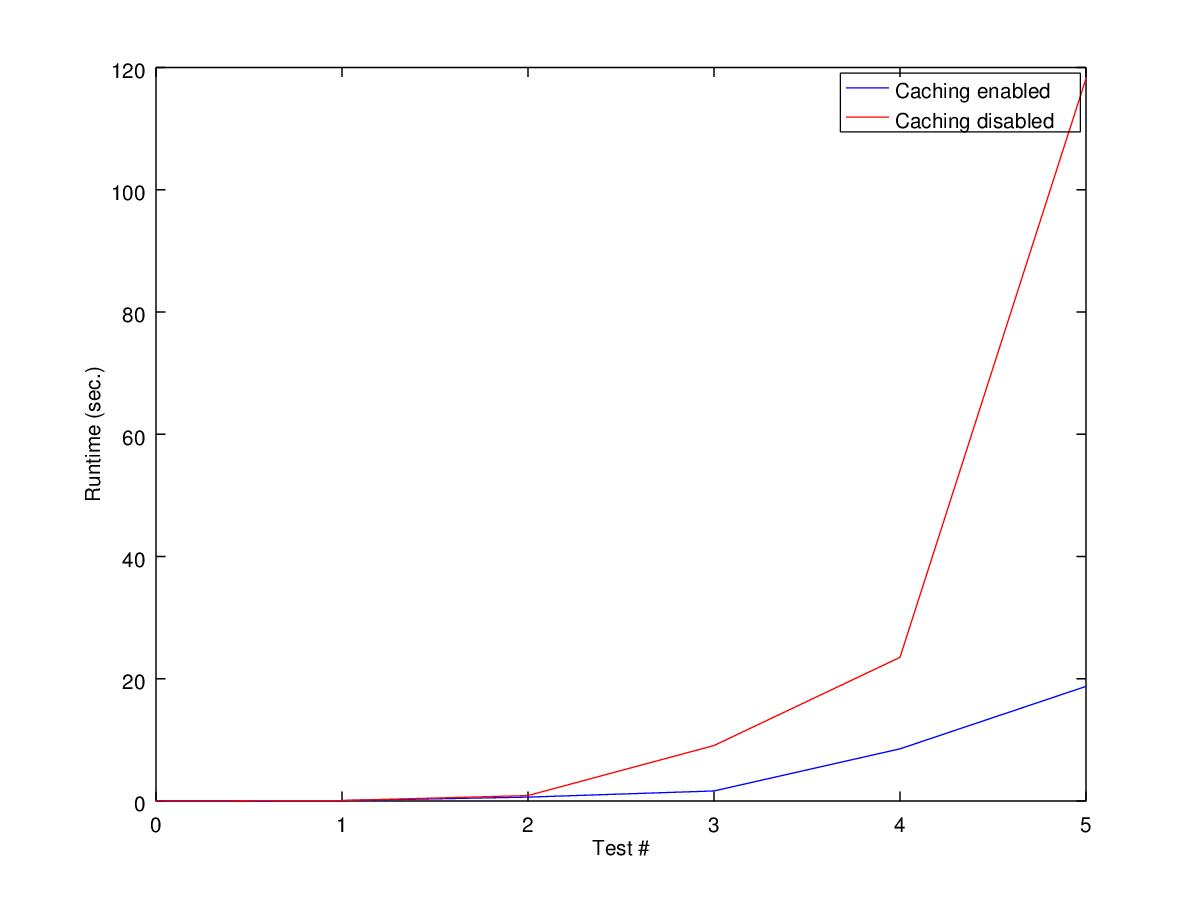
\includegraphics[width=.55\columnwidth]{resources/caching_performance.jpg}
			\captionof{figure}{Performance with/without caching \\\textit{file: resources/caching\_performance.jpg}}
			\label{fig:fig3}
		\end{figure}

		\subsubsection{Cache size}
			Caching size also makes a significant different, but only up to the number of possible paths. We do not let variable cache sizes,
			since that is too hard to benchmark. Instead, we cap the cache size at $100,000$. This accomodates for a total number of $\frac{ceil(sqrt(100000))}{2} = 159$ vertices
			all connected to each other (all possible paths). However, a map of 159x159, which has every vertex connected to every other is \textbf{very} unlikely. Below in Figure ~\ref{fig:fig4}
			you can see the effect of cache size on a map of 300x300 with several experiments, average of 3 results taken for each cache size.
		
			\begin{figure}[H]
			\centering
				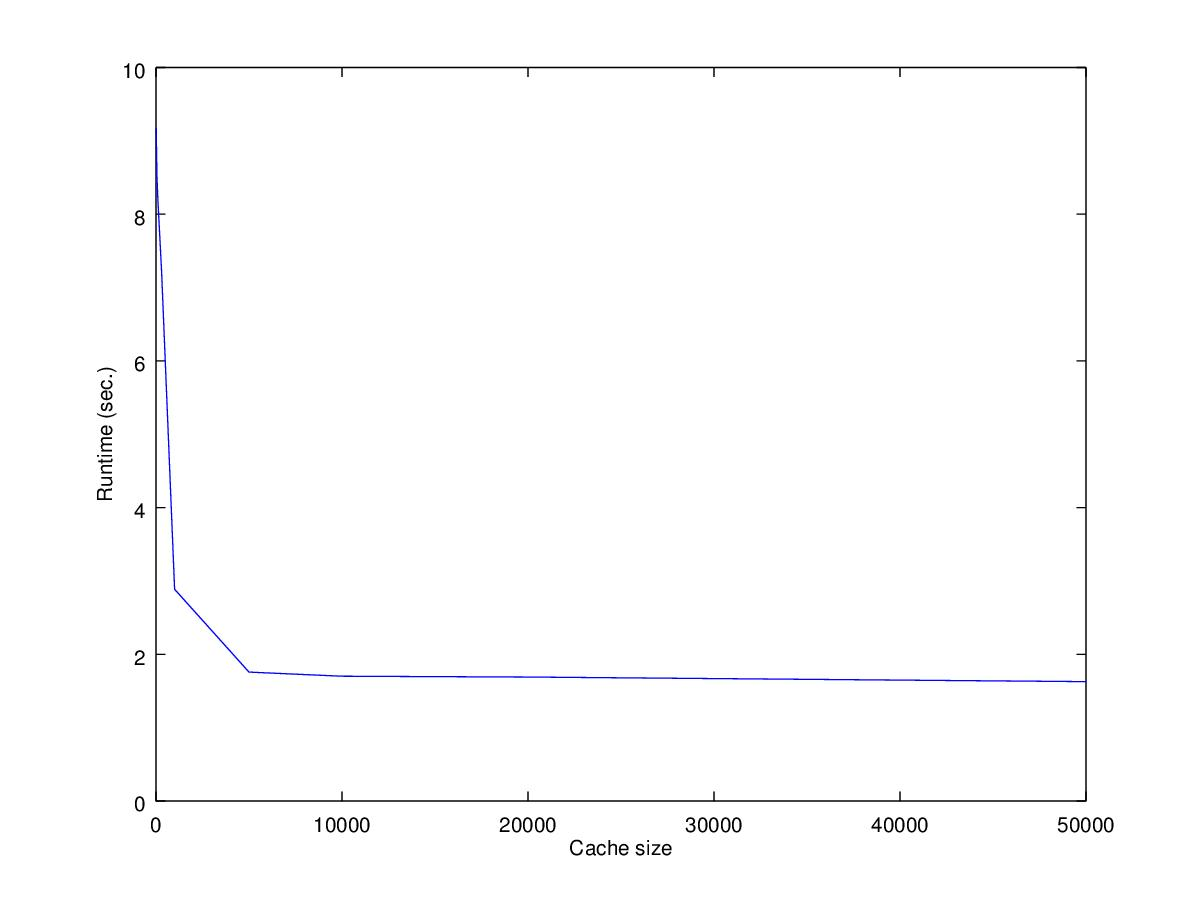
\includegraphics[width=.55\columnwidth]{resources/cache_size.jpg}
				\captionof{figure}{Effects of cache size on performance \\\textit{file: resources/cache\_size.jpg}}
				\label{fig:fig4}
			\end{figure}
			

	\section{Simulation Results} \label{stats}

		\subsection{Test inputs}
			To evaluate the simulation, two distinct input files were used. They model two different realistic scenarious.
			The first one (\textit{Three Neighborhoods}) \footnote{File: test/inputs/statistics\_collection/three\_neighborhoods.txt} models three separate connected neighborhoods, where the paths
			within the neighborhoods are shorter than the path between them. (See figure~\ref{fig:fig5a}) 
			\\
			\\
			The second input (\textit{Big Cluster}) \footnote{File: test/inputs/statistics\_collection/big\_cluster.txt} models one big area where all of the bins are interconnected and paths
			within it are comparable in distance/duration. (See figure~\ref{fig:fig5b})
			\\
			\\
			We expect the priority algorithm, which selects bins based on their distance from the current location, to work
			better on the \textit{Three neighborhoods} area and for them to work comparably well on the big cluster area.

			\begin{figure}[H]
				\centering
				\begin{subfigure}[b]{.5\textwidth}
					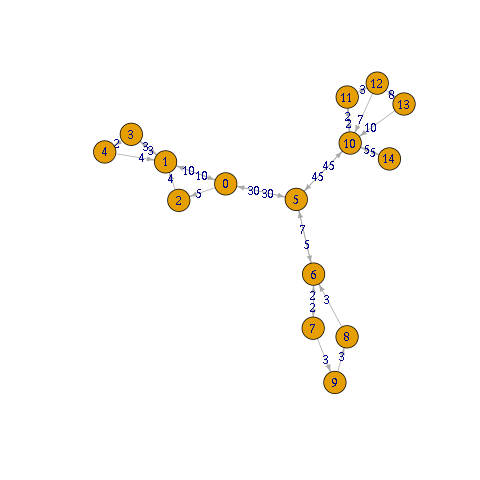
\includegraphics[width=\textwidth]{resources/three_neighborhoods.png}
					\caption{Three Neighborhoods \\\textit{file: resources/three\_neighborhoods.png}}
					\label{fig:fig5a}
				\end{subfigure}\hfill%
				\begin{subfigure}[b]{.5\textwidth}
					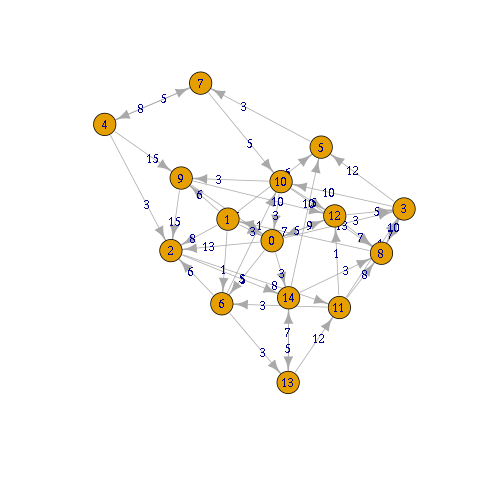
\includegraphics[width=\textwidth]{resources/big_cluster.png}
					\caption{Big Cluster \\\textit{file: resources/three\_neighborhoods.png}}
					\label{fig:fig5b}
				\end{subfigure}
				\label{fig:fig5}
				\caption{Areas used for evaluation}
			\end{figure}

		\subsection{Bin Occupancy Evolution}
		The first metric of interest is the bin volume plotted against time. In figure~\ref{fig:fig6a} and figure~\ref{fig:fig6b} we
		can see the average volume of the bins for the \textit{Three Neighborhoods} and \textit{Big Cluster} areas. In both
		$disposalDistrShape\ =\ 3$ (3 bags per hour) and $serviceFreq = 0.04167$ (one service daily), but in ~\ref{fig:fig6a}
		$disposalDistrRate\ = \ 5.0$, while in ~\ref{fig:fig6b} $disposalDistrRate\ =\ 3$. Both of the simulations stop after
		a week with a warm-up time of a day and both have a bag volume of $0.05$ with a maximum bin volume of $2$.
		\\
		\\
		Since the mean of the Erlang-K distribution is $\mu\ =\ \frac{k}{\lambda}$, in each case we would expect the average bin content
		before each service period to follow:
    	\begin{equation}
			bin\_content\ =\ \frac{time\_between\_service\_periods}{\mu_{erlang}}\ *\ bin\_volume
		\end{equation}
		\\
		\\
		Given that all bins are independent\footnote{By the specifications}. This yields $1.8\ m^3$ average volume for \textit{Three Neighborhoods}
		and $3\ m^3$ for \textit{Big Cluster}, which is what is observed in the graphs. Note, however, that the bins cannot have a maximum volume of
		$2\ m^3$, therefore on the second graph we see the "cap".


		\begin{figure}[H]
			\centering
			\begin{subfigure}[b]{.5\columnwidth}
				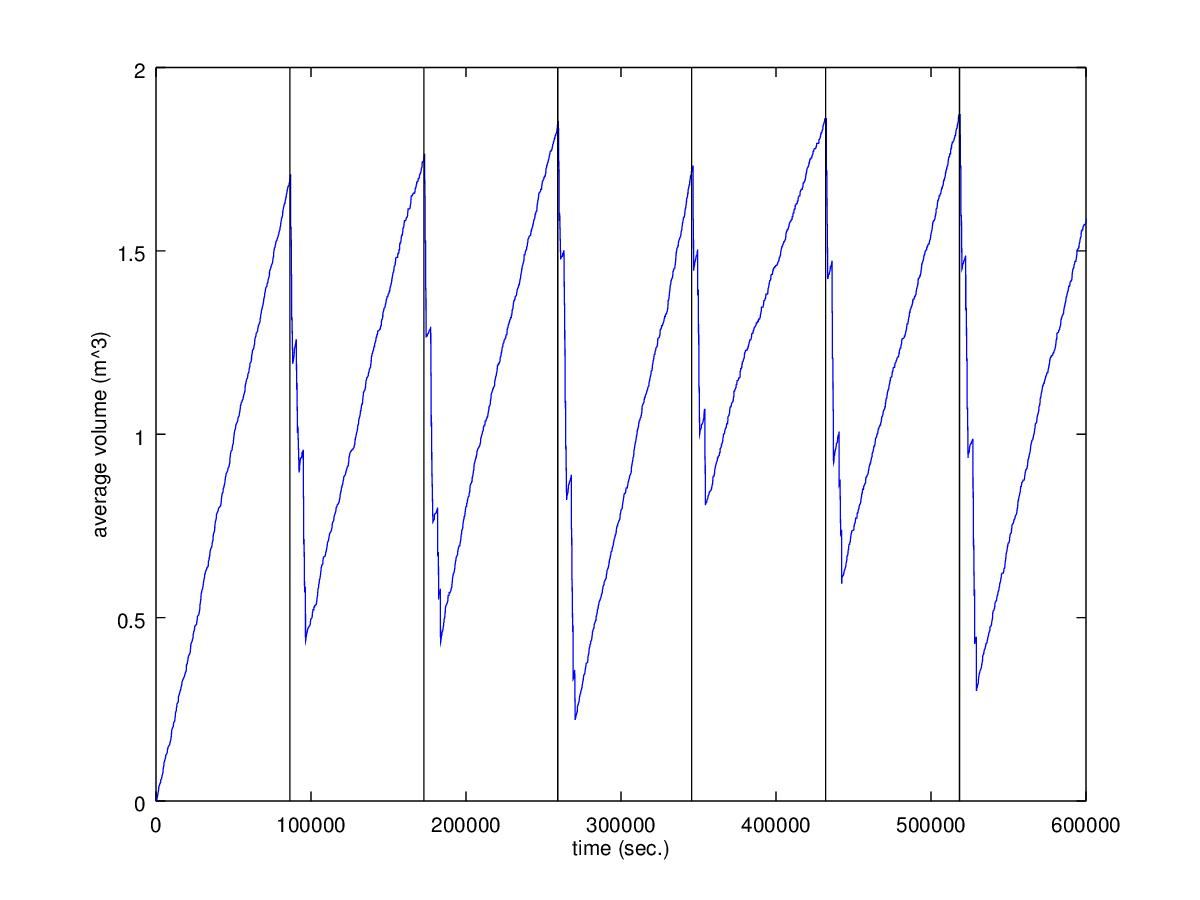
\includegraphics[width=\textwidth]{resources/occupancy_three_neighborhoods.jpg}
				\caption{Bin Volume Evolution (Three Neighborhoods) \\\textit{file: resources/occupancy\_three\_neighborhoods.png}}
				\label{fig:fig6a}
			\end{subfigure}\hfill%
			\begin{subfigure}[b]{.5\columnwidth}
				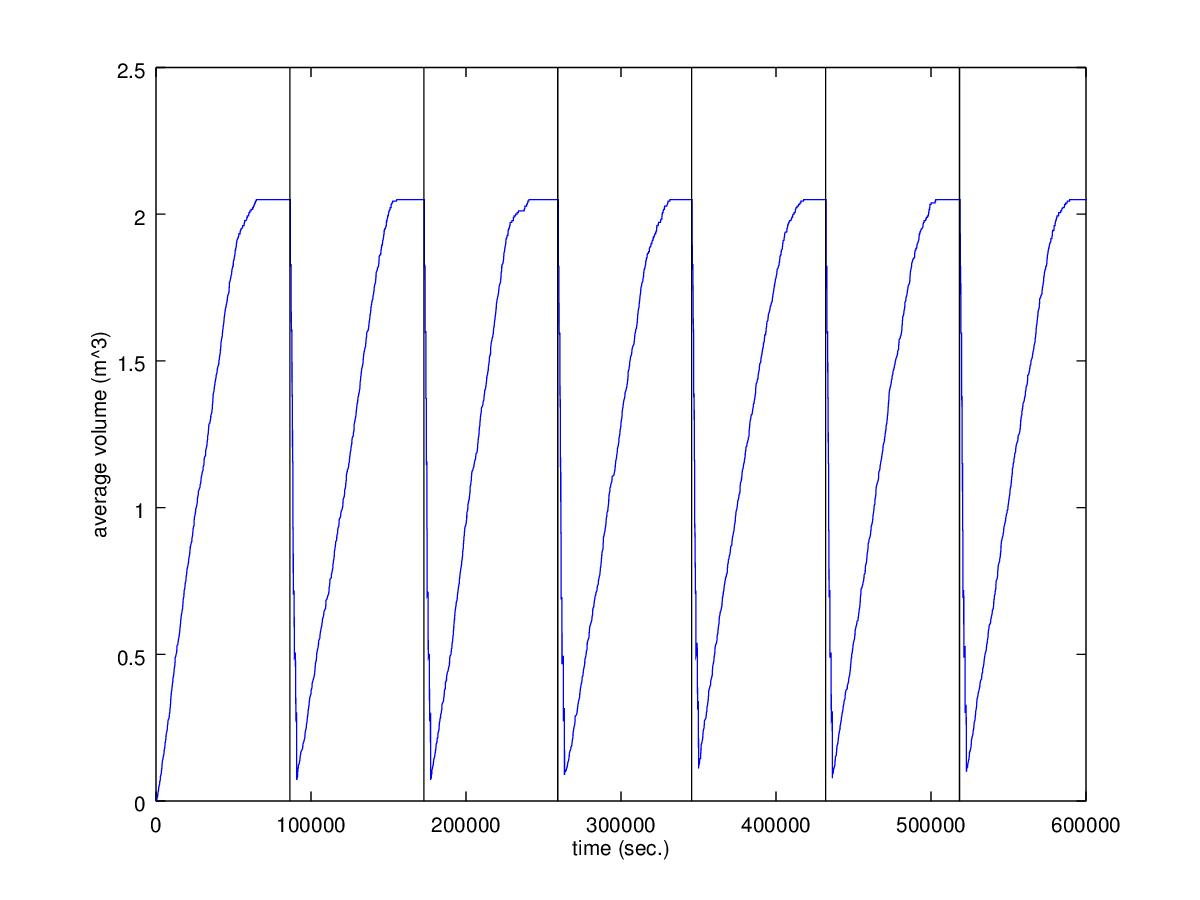
\includegraphics[width=\textwidth]{resources/occupancy_big_cluster.jpg}
				\caption{Bin Volume Evolution (Big Cluster) \\\textit{file: resources/occupancy\_big\_cluster.png}}
				\label{fig:fig6b}
			\end{subfigure}
			\label{fig:fig6}
		\end{figure}


		\subsection{Trip Efficiency}
		The first metric is trip effiency. For figure ~\ref{fig:fig7a}, ~\ref{fig:fig7b} we hold $distributionShape\ =\ 2$, $serviceFreq = 0.0416$ (once a day) and vary $distributionRate$, recording
		the trip efficiency for both \textit{Three Neighborhoods} and \textit{Big Cluster}.
		

		\begin{figure}[H]
			\centering
			\begin{subfigure}[b]{.5\textwidth}
				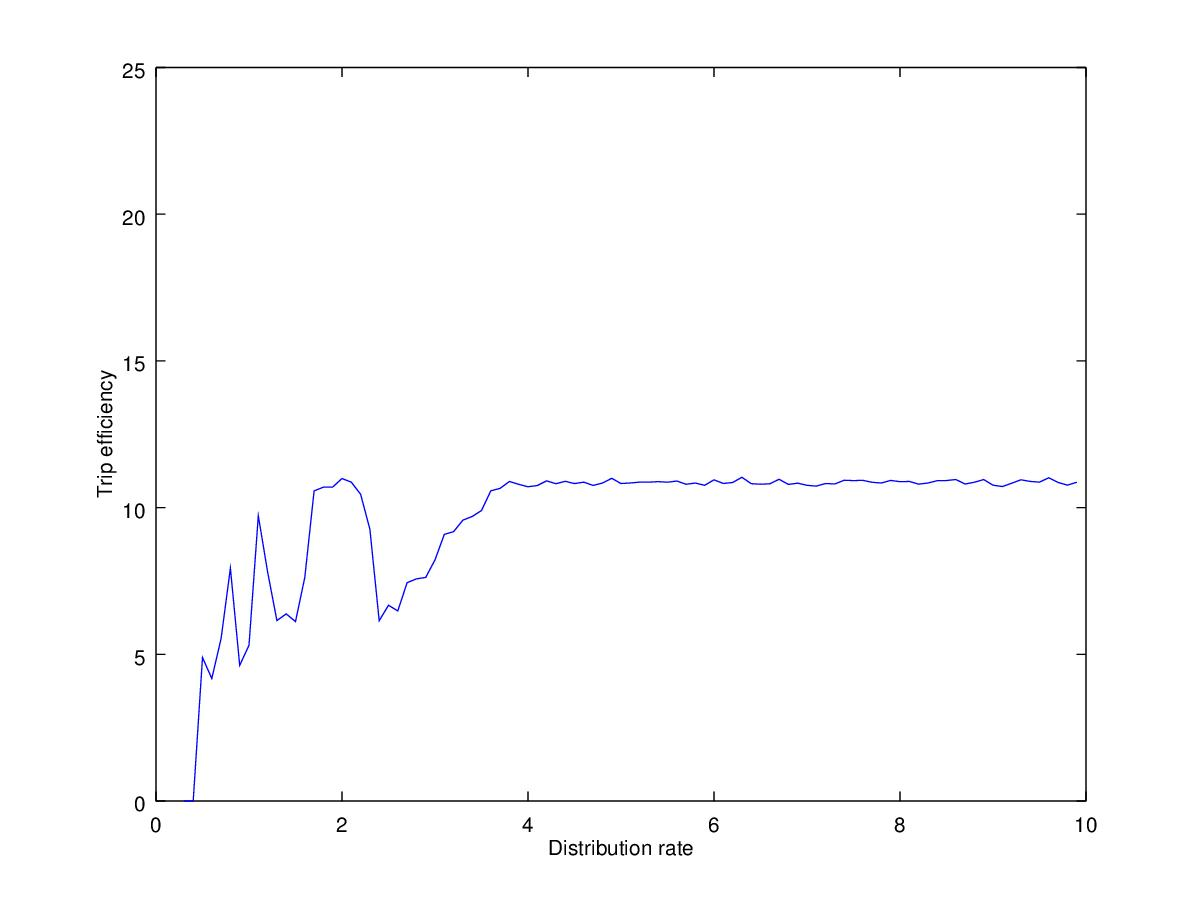
\includegraphics[width=\textwidth]{resources/three_neighborhoods_dist_rate_trip_eff.jpg}
				\caption{Three Neighborhoods \\\textit{file: resources/three\_neighborhoods\_dist\_rate\_trip\_eff.jpg}}
				\label{fig:fig7a}
			\end{subfigure}\hfill%
			\begin{subfigure}[b]{.5\textwidth}
				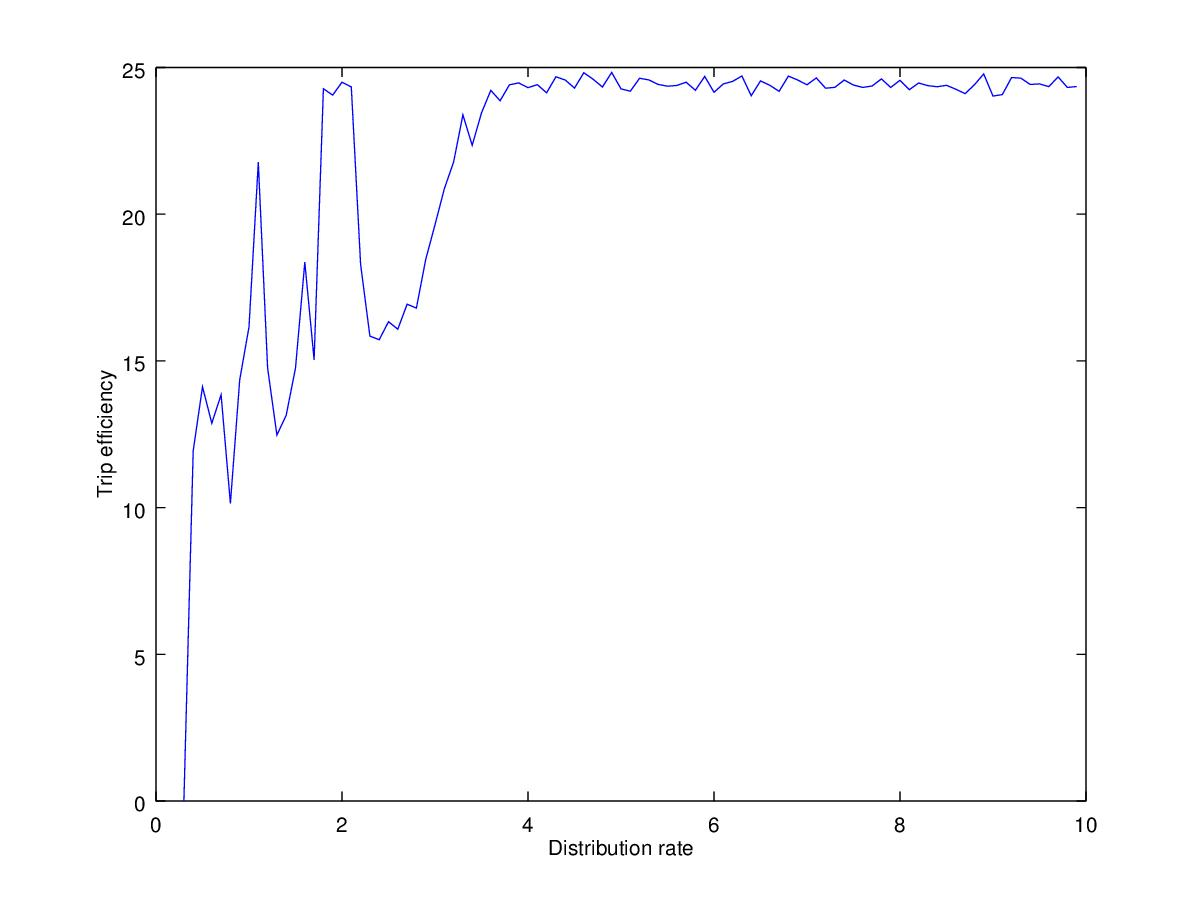
\includegraphics[width=\textwidth]{resources/big_cluster_dist_rate_trip_eff.jpg}
				\caption{Big Cluster\\\textit{file: resources/big\_cluster\_dist\_rate\_trip\_eff.jpg}}
				\label{fig:fig7b}
			\end{subfigure}
			\label{fig:fig7}
			\caption{Trip Efficiency/Distribution Rate}
		\end{figure}


		\subsection{Bin Overflow}
		\begin{figure}[H]
			\centering
			\begin{subfigure}[b]{.5\textwidth}
				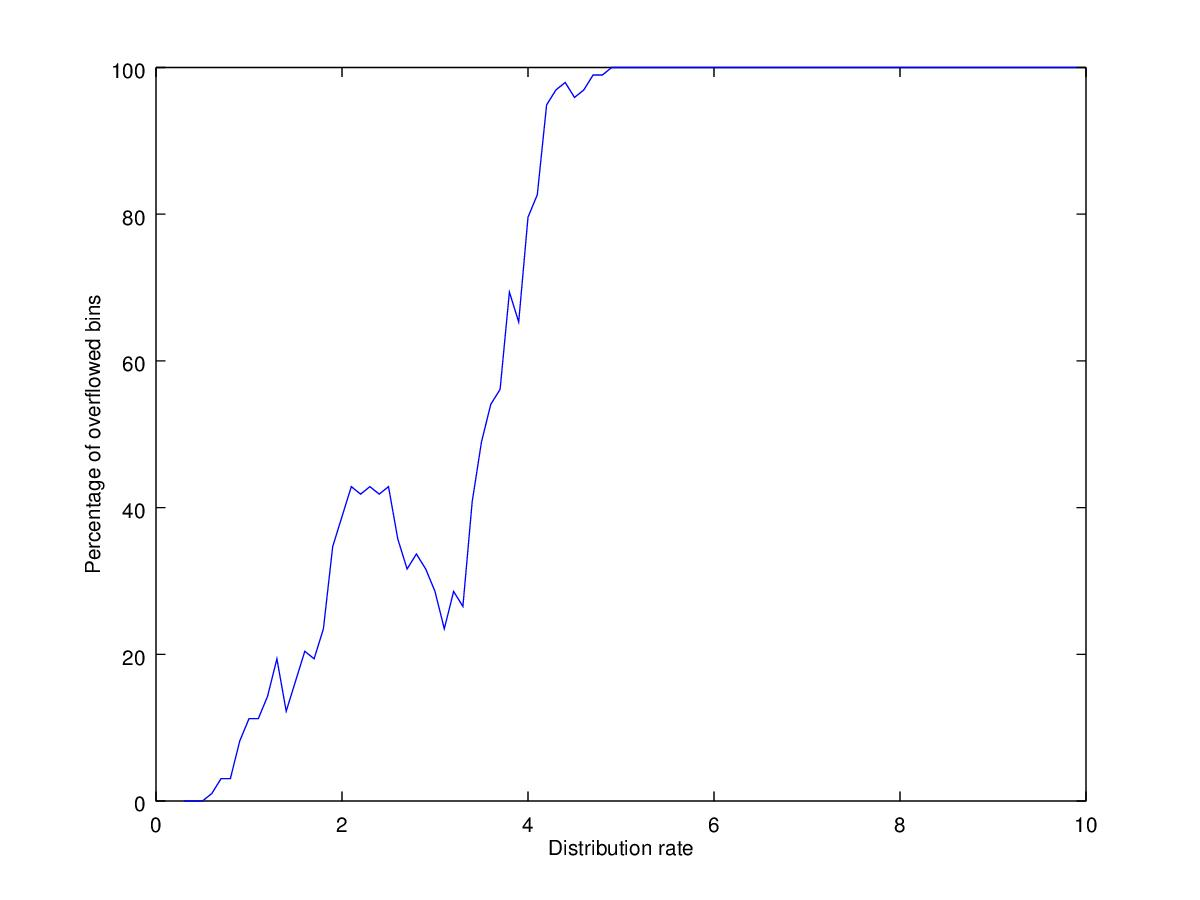
\includegraphics[width=\textwidth]{resources/three_neighborhoods_dist_rate_overflow.jpg}
				\caption{Three Neighborhoods \\\textit{file: resources/three\_neighborhoods\_dist\_rate\_overflow.jpg}}
				\label{fig:fig8a}
			\end{subfigure}\hfill%
			\begin{subfigure}[b]{.5\textwidth}
				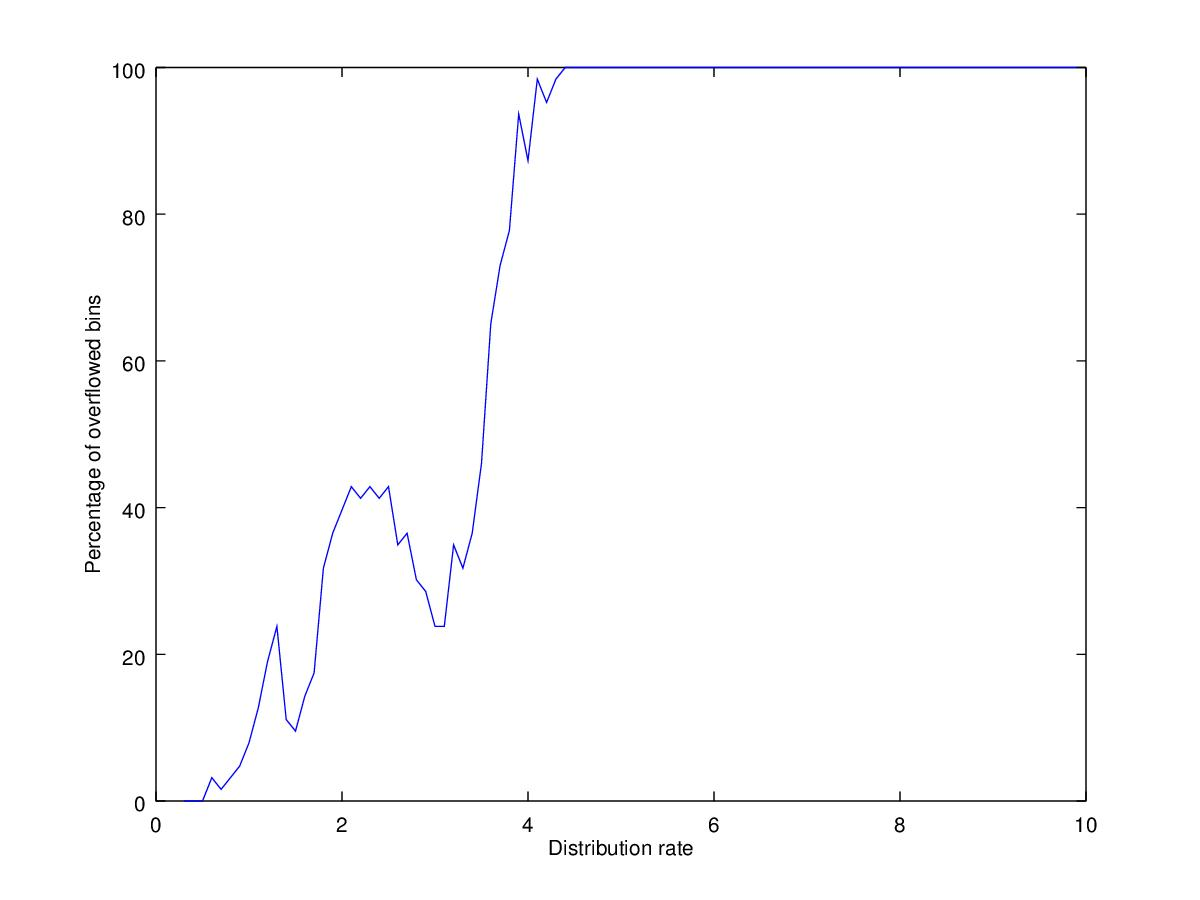
\includegraphics[width=\textwidth]{resources/big_cluster_dist_rate_overflow.jpg}
				\caption{Big Cluster\\\textit{file: resources/big\_cluster\_dist\_rate\_overflow.jpg}}
				\label{fig:fig8b}
			\end{subfigure}
			\label{fig:fig8}
			\caption{Bin overflow percentage/Distribution Rate}
		\end{figure}


		\subsection{Algorithm Efficiency}
		The last metric is the efficiency as archieved by the greedy and priority algorithms. We measure efficiency
		against service frequency, holding $distributionShape\ =\ 2$ and  $distributionRate = 3.0$. We would expect 
		trip effiency to go down as the service frequency increases, but also the priority algorithm to perform better
		than the greedy one on the \textit{Three neighborhoods} area.

		\begin{figure}[H]
			\centering
			\begin{subfigure}[b]{.5\textwidth}
				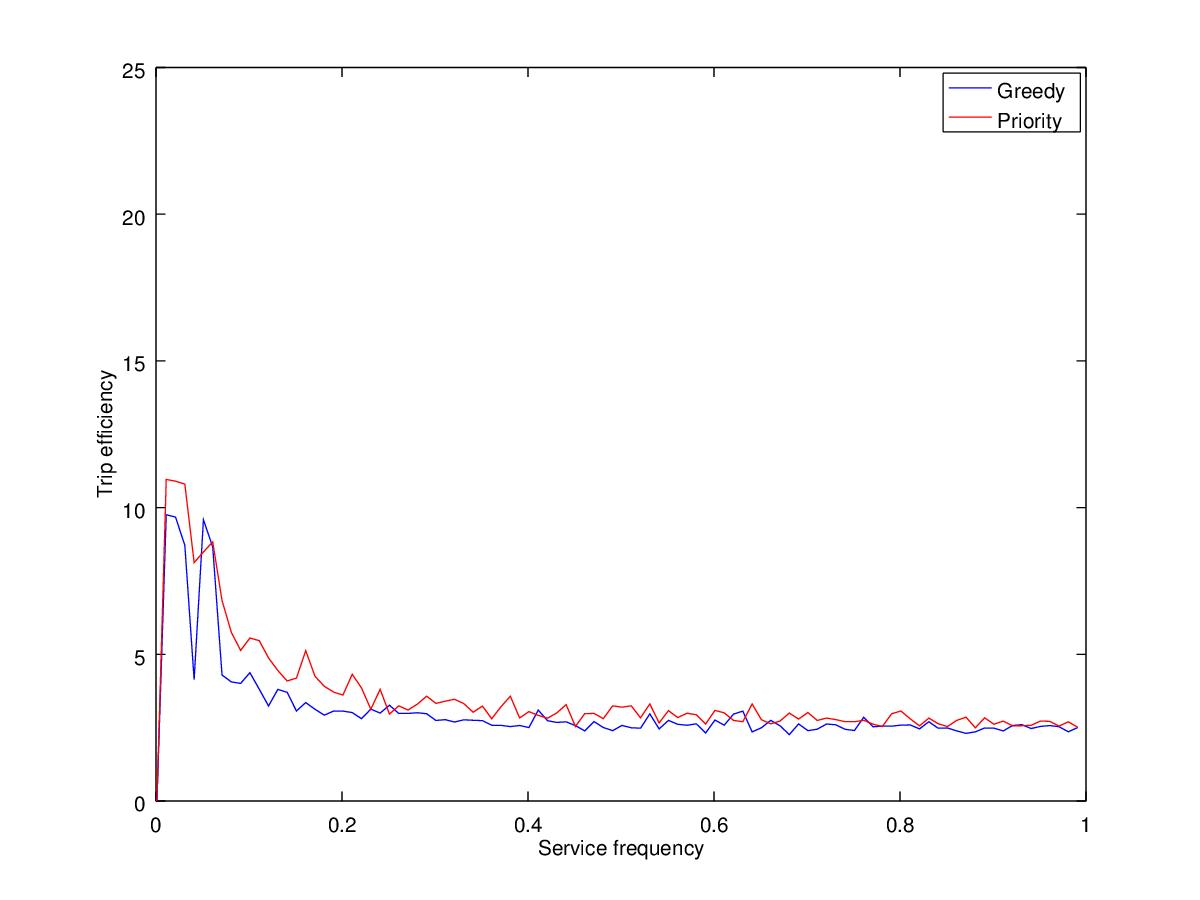
\includegraphics[width=\textwidth]{resources/three_neighborhoods_service_freq_trip_eff_algo.jpg}
				\caption{Three Neighborhoods \\\textit{file: resources/three\_neighborhoods\_service\_freq\_trip\_eff\_algo.jpg}}
				\label{fig:fig9a}
			\end{subfigure}\hfill%
			\begin{subfigure}[b]{.5\textwidth}
				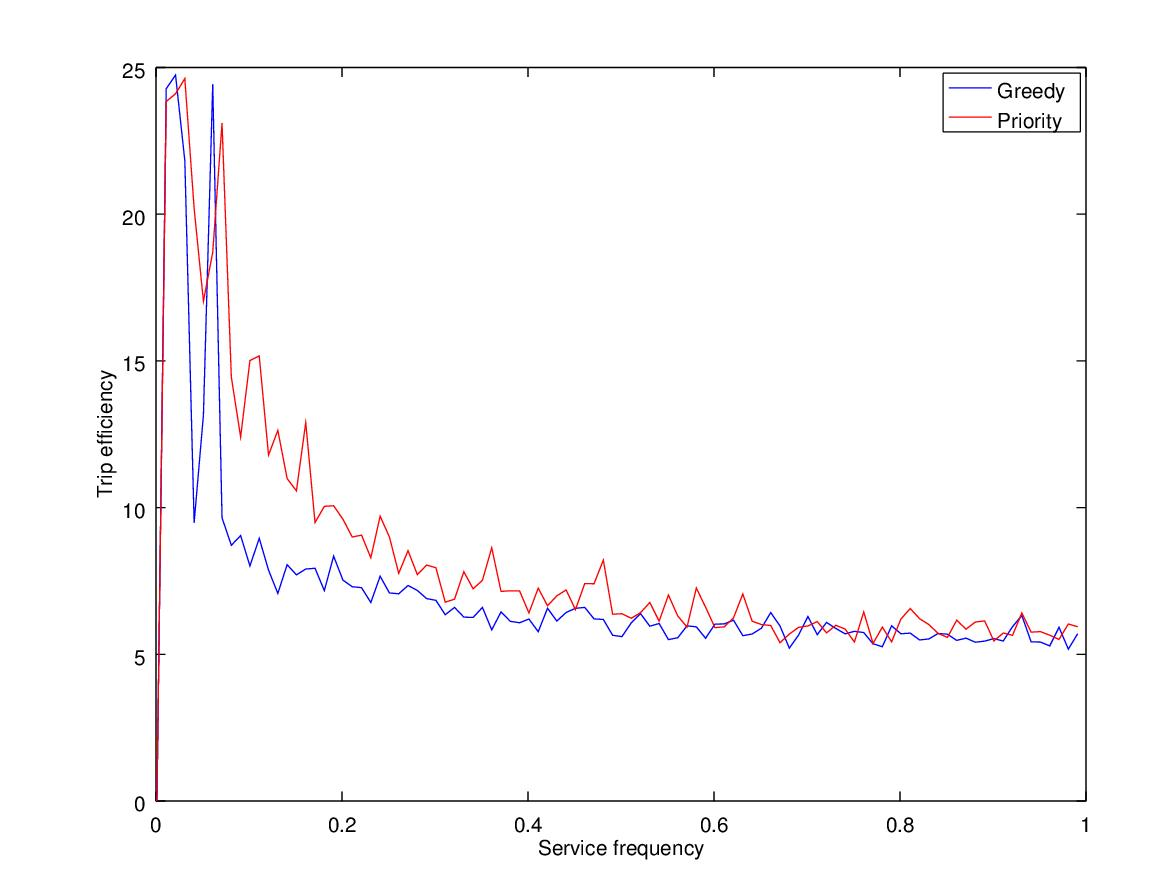
\includegraphics[width=\textwidth]{resources/big_cluster_service_freq_trip_eff_algo.jpg}
				\caption{Big Cluster\\\textit{file: resources/big\_cluster\_service\_freq\_trip\_eff\_algo.jpg}}
				\label{fig:fig9b}
			\end{subfigure}
			\label{fig:fig9}
			\caption{Effiency/Service Frequency}
		\end{figure}

		\subsection{Analysis}
		Trip efficiency increases as the distribution rate increases. They are positively correlated, though
		as the lorry reaches its maximum efficiency, no matter how much more bags are disposed and bins overflow,
		the efficiency doesn't increase.
		
		\begin{equation}
			\sigma(dist\_rate,\ efficiency)\ = 0.66919
		\end{equation} 

		Naturally, as we add more garbage to the system, the bins start to overflow more, thus trip efficiency alone
		is a poor metric of the overall efficiency of the system. We can see that bins overflowing also correlate with
		the distribution shape (and more strongly so than efficiency):

		\begin{equation}
			\sigma(dist\_rate,\ percentage\_bins\_overflowing) = 0.87768
		\end{equation}

		We also note that trip efficiency is generally poor on areas such as \textit{Three Neighborhoods}, since
		the distance between neighborhoods is much bigger that the one within a neighborhood and a lorry servicing
		more than one neighborhood would have to make trips around the long edges in the graph.
		For this reason, however, \textbf{priority} Dijkstra performs better than its \textbf{greedy} counterpart.
		Since making a trip to a different neighborhood is expensive, visiting bins close together first is generally
		a good idea. However, even the smarter algorithm cannot do anything when the bins that need servicing are
		spread out between areas, which might explain why the difference in efficiency is not that big.
		An intersting thing to note is that as the service rate goes up to one an hour almost no bins will need
		servicing, hence at the very extreme both algorithms would achieve the same efficiency (the extreme being only
		one bin that needs servicing at every schedule).

		\section{Testing}
		The majority of testing is automated using \textit{pyunit} and separate test cases for each class in the application.
		Performance testing was done somewhat differently, where output was disabled via a command line flag (\textit(-bod)) and
		multiple runs were performed using specially generated files (as discussed below). In addition, the aforementioned \textit{Three Neighborhoods}
		and \textit{Big Cluster} areas have 2 input files each, describing just the area or the area with experiments, as used in the 
		previous section for analysis.

		\subsection{Automated Testing}
		Automated testing is divided into a single test suite (single file) that tests one class and within that test suite many test
		cases. Here is an outline of the test cases, for more information each suite has appropriate documentation. The location of all
		unit tests is \textit{test/<name>\_test.py}.

		\begin{itemize}
			\item \textit{area\_test.py} \- Tests area functionality, including disposal events generation, route planning
				and proper usage of the \textit{EventDispatcher} class. Includes edge cases for lorry overflow and resheduling.
			
			\item \textit{dijkstra\_route\_planner\_test.py} \- Test the route planning algorithm, both the greedy and priority version.
			
			\item \textit{event\_dispatcher\_test.py} \- Tests that the \textit{EventDispatcher} class stores and execues events
				in the correct order.

			\item \textit{input\_parser\_test.py} \- Contains various tests for the \textit{InputParser}, including valid and invalid
				files. All of the files in \textit{test/inputs/parser\_tests} are used here.

			\item \textit{output\_formatter\_test.py} \- Tests that the output formatter correctly displays events by watching the standard
				output.

			\item \textit{statistics\_aggregator\_test.py} \- General statistics tests for the aggregator class.
		\end{itemize}

		\subsection{Sample inputs}
		\subsubsection{Input Parser}
		Sample inputs are in \textit{test/inputs/parser\_tests}. Check the corresponding test suite for a morecomprehensive description
		of each test and expected results.
	
		\subsubsection{Performance testing} \label{performance}
		The above performance tests (section ~\ref{optimization})) were all done using inputs in \textit{test/inputs/performance\_tests}.
		Each area input was generated via the script file \textit{test/generate\_performance\_test.py}. Performance testing was done
		using three area sizes and experimentation.
		\\
		\\
		The following are the tests (ordered by \textit{Test \#}), as performed in ascending order (from fastest to slowest).
		\begin{enumerate}[start=0]
			\item \textit{small\_area.txt} \- 5x5 area, no experiments
			\item \textit{small\_area\_experiments.txt} \- 5x5 area, 4 experiments
			\item \textit{medium\_area.txt} \- 50x50 area, no experiments
			\item \textit{medium\_area\_experiments.txt} \- 5x5 area, 4 experiments
			\item \textit{big\_area.txt} \- 300x300 area, no experiments
			\item \textit{big\_area\_experiments.txt} \- A 300x300 area, all vertices connected, 4 experiments. Runtimes should be slowest here.
		\end{enumerate}

		\subsubsection{Statistics collection}
		The tests used in Section ~\ref{stats} are all in \textit{inputs/statistics\_collection}. There are two files for each area,
		one with experiments and one without. Since more than one experiments were run, both files contain all the experiment data.
		If you wish to replicate, a good idea might be to comment some of the experiments out.

		\section{Conclusion}
		The algorithm used for this simulation performed reasonably well and with caching can scale effectively. In a small to medium scale scenario
		the simulator has reasonable runtimes and no issues dealing with complicated networks. However, a different approach
		using $A^*$ and a custom heuristic, perhaps combining both of the heuristics used here could yield better results. Additionally, it would
		be beneficial if the simulation was run on areas derived from actual maps of cities and the above statistics recorded. For larger areas,
		the simulation could benefit from a parallel architecture, where different areas are run on different threads/simultaneously.

		\section{Resources}
		\begin{itemize}
			\item Graphs plotted using \textit{R}, other plots using \textit{Octave}. All scripts used for plotting are in \textit{/statistics\_plots}
		\end{itemize}

\end{document}
